\documentclass[]{article}
\usepackage{lmodern}
\usepackage{amssymb,amsmath}
\usepackage{ifxetex,ifluatex}
\usepackage{fixltx2e} % provides \textsubscript
\ifnum 0\ifxetex 1\fi\ifluatex 1\fi=0 % if pdftex
  \usepackage[T1]{fontenc}
  \usepackage[utf8]{inputenc}
\else % if luatex or xelatex
  \ifxetex
    \usepackage{mathspec}
  \else
    \usepackage{fontspec}
  \fi
  \defaultfontfeatures{Ligatures=TeX,Scale=MatchLowercase}
\fi
% use upquote if available, for straight quotes in verbatim environments
\IfFileExists{upquote.sty}{\usepackage{upquote}}{}
% use microtype if available
\IfFileExists{microtype.sty}{%
\usepackage{microtype}
\UseMicrotypeSet[protrusion]{basicmath} % disable protrusion for tt fonts
}{}
\usepackage[margin=1in]{geometry}
\usepackage{hyperref}
\hypersetup{unicode=true,
            pdftitle={Analysis of bootcamp survey},
            pdfauthor={Rick Gilmore},
            pdfborder={0 0 0},
            breaklinks=true}
\urlstyle{same}  % don't use monospace font for urls
\usepackage{color}
\usepackage{fancyvrb}
\newcommand{\VerbBar}{|}
\newcommand{\VERB}{\Verb[commandchars=\\\{\}]}
\DefineVerbatimEnvironment{Highlighting}{Verbatim}{commandchars=\\\{\}}
% Add ',fontsize=\small' for more characters per line
\usepackage{framed}
\definecolor{shadecolor}{RGB}{248,248,248}
\newenvironment{Shaded}{\begin{snugshade}}{\end{snugshade}}
\newcommand{\KeywordTok}[1]{\textcolor[rgb]{0.13,0.29,0.53}{\textbf{#1}}}
\newcommand{\DataTypeTok}[1]{\textcolor[rgb]{0.13,0.29,0.53}{#1}}
\newcommand{\DecValTok}[1]{\textcolor[rgb]{0.00,0.00,0.81}{#1}}
\newcommand{\BaseNTok}[1]{\textcolor[rgb]{0.00,0.00,0.81}{#1}}
\newcommand{\FloatTok}[1]{\textcolor[rgb]{0.00,0.00,0.81}{#1}}
\newcommand{\ConstantTok}[1]{\textcolor[rgb]{0.00,0.00,0.00}{#1}}
\newcommand{\CharTok}[1]{\textcolor[rgb]{0.31,0.60,0.02}{#1}}
\newcommand{\SpecialCharTok}[1]{\textcolor[rgb]{0.00,0.00,0.00}{#1}}
\newcommand{\StringTok}[1]{\textcolor[rgb]{0.31,0.60,0.02}{#1}}
\newcommand{\VerbatimStringTok}[1]{\textcolor[rgb]{0.31,0.60,0.02}{#1}}
\newcommand{\SpecialStringTok}[1]{\textcolor[rgb]{0.31,0.60,0.02}{#1}}
\newcommand{\ImportTok}[1]{#1}
\newcommand{\CommentTok}[1]{\textcolor[rgb]{0.56,0.35,0.01}{\textit{#1}}}
\newcommand{\DocumentationTok}[1]{\textcolor[rgb]{0.56,0.35,0.01}{\textbf{\textit{#1}}}}
\newcommand{\AnnotationTok}[1]{\textcolor[rgb]{0.56,0.35,0.01}{\textbf{\textit{#1}}}}
\newcommand{\CommentVarTok}[1]{\textcolor[rgb]{0.56,0.35,0.01}{\textbf{\textit{#1}}}}
\newcommand{\OtherTok}[1]{\textcolor[rgb]{0.56,0.35,0.01}{#1}}
\newcommand{\FunctionTok}[1]{\textcolor[rgb]{0.00,0.00,0.00}{#1}}
\newcommand{\VariableTok}[1]{\textcolor[rgb]{0.00,0.00,0.00}{#1}}
\newcommand{\ControlFlowTok}[1]{\textcolor[rgb]{0.13,0.29,0.53}{\textbf{#1}}}
\newcommand{\OperatorTok}[1]{\textcolor[rgb]{0.81,0.36,0.00}{\textbf{#1}}}
\newcommand{\BuiltInTok}[1]{#1}
\newcommand{\ExtensionTok}[1]{#1}
\newcommand{\PreprocessorTok}[1]{\textcolor[rgb]{0.56,0.35,0.01}{\textit{#1}}}
\newcommand{\AttributeTok}[1]{\textcolor[rgb]{0.77,0.63,0.00}{#1}}
\newcommand{\RegionMarkerTok}[1]{#1}
\newcommand{\InformationTok}[1]{\textcolor[rgb]{0.56,0.35,0.01}{\textbf{\textit{#1}}}}
\newcommand{\WarningTok}[1]{\textcolor[rgb]{0.56,0.35,0.01}{\textbf{\textit{#1}}}}
\newcommand{\AlertTok}[1]{\textcolor[rgb]{0.94,0.16,0.16}{#1}}
\newcommand{\ErrorTok}[1]{\textcolor[rgb]{0.64,0.00,0.00}{\textbf{#1}}}
\newcommand{\NormalTok}[1]{#1}
\usepackage{graphicx,grffile}
\makeatletter
\def\maxwidth{\ifdim\Gin@nat@width>\linewidth\linewidth\else\Gin@nat@width\fi}
\def\maxheight{\ifdim\Gin@nat@height>\textheight\textheight\else\Gin@nat@height\fi}
\makeatother
% Scale images if necessary, so that they will not overflow the page
% margins by default, and it is still possible to overwrite the defaults
% using explicit options in \includegraphics[width, height, ...]{}
\setkeys{Gin}{width=\maxwidth,height=\maxheight,keepaspectratio}
\IfFileExists{parskip.sty}{%
\usepackage{parskip}
}{% else
\setlength{\parindent}{0pt}
\setlength{\parskip}{6pt plus 2pt minus 1pt}
}
\setlength{\emergencystretch}{3em}  % prevent overfull lines
\providecommand{\tightlist}{%
  \setlength{\itemsep}{0pt}\setlength{\parskip}{0pt}}
\setcounter{secnumdepth}{0}
% Redefines (sub)paragraphs to behave more like sections
\ifx\paragraph\undefined\else
\let\oldparagraph\paragraph
\renewcommand{\paragraph}[1]{\oldparagraph{#1}\mbox{}}
\fi
\ifx\subparagraph\undefined\else
\let\oldsubparagraph\subparagraph
\renewcommand{\subparagraph}[1]{\oldsubparagraph{#1}\mbox{}}
\fi

%%% Use protect on footnotes to avoid problems with footnotes in titles
\let\rmarkdownfootnote\footnote%
\def\footnote{\protect\rmarkdownfootnote}

%%% Change title format to be more compact
\usepackage{titling}

% Create subtitle command for use in maketitle
\newcommand{\subtitle}[1]{
  \posttitle{
    \begin{center}\large#1\end{center}
    }
}

\setlength{\droptitle}{-2em}

  \title{Analysis of bootcamp survey}
    \pretitle{\vspace{\droptitle}\centering\huge}
  \posttitle{\par}
    \author{Rick Gilmore}
    \preauthor{\centering\large\emph}
  \postauthor{\par}
      \predate{\centering\large\emph}
  \postdate{\par}
    \date{2018-07-25 08:38:00}


\begin{document}
\maketitle

{
\setcounter{tocdepth}{3}
\tableofcontents
}
\subsection{Goals}\label{goals}

\begin{itemize}
\tightlist
\item
  Download and clean data from 2018 R Bootcamp Survey
\item
  Visualize data
\item
  Prepare reports in \texttt{ioslides\_presentation},
  \texttt{pdf\_document}, and \texttt{word\_document} formats
\end{itemize}

\subsection{Preliminaries}\label{preliminaries}

Load required packages.

\begin{Shaded}
\begin{Highlighting}[]
\KeywordTok{library}\NormalTok{(tidyverse)}
\KeywordTok{library}\NormalTok{(googlesheets)}
\end{Highlighting}
\end{Shaded}

\subsection{Load data and examine}\label{load-data-and-examine}

The survey data are stored in a
\href{https://docs.google.com/spreadsheets/d/1-YB0iWUNN_9oxBhz221NFiyBOcwMfHziFeUiUvQwn7k/edit\#gid=2108979913}{Google
Sheet}. We'll use the \texttt{googlesheets} package to open it and
create a data frame. Documentation about the package can be found
\href{https://cran.r-project.org/web/packages/googlesheets/vignettes/basic-usage.html}{here}.

There are some idiosyncrasies in using the \texttt{googlesheets} package
in an R Markdown document because it requires interaction with the
console, so I created a separate R script,
\texttt{Get\_bootcamp\_googlesheet.R} to extract the survey data. If you
try to execute the next chunk, it may give you an error, or it may ask
you to allow \texttt{googlesheets} to access information in your Google
profile.

\begin{verbatim}
survey_url <- "https://docs.google.com/spreadsheets/d/1-YB0iWUNN_9oxBhz221NFiyBOcwMfHziFeUiUvQwn7k/edit?usp=sharing"

bootcamp_by_url <- survey_url %>%
  googlesheets::extract_key_from_url() %>%
  googlesheets::gs_key()

bootcamp_sheets <- gs_ws_ls(bootcamp_by_url)

boot_data <- bootcamp_by_url %>%
  gs_read(bootcamp_sheets[1])
          
write_csv(boot_data, path=params$data_file_out)
\end{verbatim}

This script downloads the data file saves it to a CSV under
../data/survey\_2018.csv. We can then load this file.

I also created a test data file, \texttt{data/survey-test.csv} so I
could see how everything worked before y'all filled out your responses.
The \href{../R/Make_test_survey.R}{\texttt{R/Make\_test\_survey.R}} file
shows how I did this. It's a great, reproducible practice to
\textbf{simulate the data you expect}, then run it through your
pipeline.

\begin{center}\rule{0.5\linewidth}{\linethickness}\end{center}

\begin{Shaded}
\begin{Highlighting}[]
\CommentTok{# Created test data set for testing.}
\NormalTok{survey <-}\StringTok{ }\KeywordTok{read_csv}\NormalTok{(params}\OperatorTok{$}\NormalTok{data_file_in)}
\end{Highlighting}
\end{Shaded}

\begin{verbatim}
## Parsed with column specification:
## cols(
##   Timestamp = col_datetime(format = ""),
##   R_exp = col_character(),
##   Banjo = col_integer(),
##   Psych_age_yrs = col_integer(),
##   Sleep_hrs = col_double(),
##   Fav_date = col_date(format = ""),
##   Crisis = col_character()
## )
\end{verbatim}

\begin{Shaded}
\begin{Highlighting}[]
\CommentTok{# Or choose data from respondents}
\CommentTok{#survey <- read_csv(data_file_in)}
\end{Highlighting}
\end{Shaded}

\begin{Shaded}
\begin{Highlighting}[]
\NormalTok{survey}
\end{Highlighting}
\end{Shaded}

\begin{verbatim}
## # A tibble: 50 x 7
##    Timestamp           R_exp   Banjo Psych_age_yrs Sleep_hrs Fav_date  
##    <dttm>              <chr>   <int>         <int>     <dbl> <date>    
##  1 2018-07-24 14:54:13 limited     4            74      6.97 2018-07-24
##  2 2018-07-24 14:54:13 some        8            27      7.74 2018-07-24
##  3 2018-07-24 14:54:13 none        3            26      6.81 2018-07-24
##  4 2018-07-24 14:54:13 limited     8            80      6.21 2018-07-24
##  5 2018-07-24 14:54:13 none        7            17      7.73 2018-07-24
##  6 2018-07-24 14:54:13 some       10            37      8.73 2018-07-24
##  7 2018-07-24 14:54:13 limited    10            46      6.67 2018-07-24
##  8 2018-07-24 14:54:13 lots        2            32      8.34 2018-07-24
##  9 2018-07-24 14:54:13 lots        3            55      7.71 2018-07-24
## 10 2018-07-24 14:54:13 lots       10            55      8.57 2018-07-24
## # ... with 40 more rows, and 1 more variable: Crisis <chr>
\end{verbatim}

The \texttt{str()} or `structure' command is also a great way to see
what you've got.

\begin{Shaded}
\begin{Highlighting}[]
\KeywordTok{str}\NormalTok{(survey)}
\end{Highlighting}
\end{Shaded}

\begin{verbatim}
## Classes 'tbl_df', 'tbl' and 'data.frame':    50 obs. of  7 variables:
##  $ Timestamp    : POSIXct, format: "2018-07-24 14:54:13" "2018-07-24 14:54:13" ...
##  $ R_exp        : chr  "limited" "some" "none" "limited" ...
##  $ Banjo        : int  4 8 3 8 7 10 10 2 3 10 ...
##  $ Psych_age_yrs: int  74 27 26 80 17 37 46 32 55 55 ...
##  $ Sleep_hrs    : num  6.97 7.74 6.81 6.21 7.73 ...
##  $ Fav_date     : Date, format: "2018-07-24" "2018-07-24" ...
##  $ Crisis       : chr  "Yes, significant" "Yes, slight" "Yes, slight" "Yes, significant" ...
##  - attr(*, "spec")=List of 2
##   ..$ cols   :List of 7
##   .. ..$ Timestamp    :List of 1
##   .. .. ..$ format: chr ""
##   .. .. ..- attr(*, "class")= chr  "collector_datetime" "collector"
##   .. ..$ R_exp        : list()
##   .. .. ..- attr(*, "class")= chr  "collector_character" "collector"
##   .. ..$ Banjo        : list()
##   .. .. ..- attr(*, "class")= chr  "collector_integer" "collector"
##   .. ..$ Psych_age_yrs: list()
##   .. .. ..- attr(*, "class")= chr  "collector_integer" "collector"
##   .. ..$ Sleep_hrs    : list()
##   .. .. ..- attr(*, "class")= chr  "collector_double" "collector"
##   .. ..$ Fav_date     :List of 1
##   .. .. ..$ format: chr ""
##   .. .. ..- attr(*, "class")= chr  "collector_date" "collector"
##   .. ..$ Crisis       : list()
##   .. .. ..- attr(*, "class")= chr  "collector_character" "collector"
##   ..$ default: list()
##   .. ..- attr(*, "class")= chr  "collector_guess" "collector"
##   ..- attr(*, "class")= chr "col_spec"
\end{verbatim}

Clearly, we need to do some cleaning before we can do anything with
this.

Let's start by renaming variables.

\begin{Shaded}
\begin{Highlighting}[]
\KeywordTok{names}\NormalTok{(survey) <-}\StringTok{ }\KeywordTok{c}\NormalTok{(}\StringTok{"Timestamp"}\NormalTok{,}
                  \StringTok{"R_exp"}\NormalTok{,}
                  \StringTok{"Banjo"}\NormalTok{,}
                  \StringTok{"Psych_age_yrs"}\NormalTok{,}
                  \StringTok{"Sleep_hrs"}\NormalTok{,}
                  \StringTok{"Fav_day"}\NormalTok{,}
                  \StringTok{"Crisis"}\NormalTok{)}
\end{Highlighting}
\end{Shaded}

\begin{Shaded}
\begin{Highlighting}[]
\CommentTok{# complete.cases() drops NAs}
\NormalTok{survey <-}\StringTok{ }\NormalTok{survey[}\KeywordTok{complete.cases}\NormalTok{(survey),]}
\NormalTok{survey}
\end{Highlighting}
\end{Shaded}

\begin{verbatim}
## # A tibble: 50 x 7
##    Timestamp           R_exp   Banjo Psych_age_yrs Sleep_hrs Fav_day   
##    <dttm>              <chr>   <int>         <int>     <dbl> <date>    
##  1 2018-07-24 14:54:13 limited     4            74      6.97 2018-07-24
##  2 2018-07-24 14:54:13 some        8            27      7.74 2018-07-24
##  3 2018-07-24 14:54:13 none        3            26      6.81 2018-07-24
##  4 2018-07-24 14:54:13 limited     8            80      6.21 2018-07-24
##  5 2018-07-24 14:54:13 none        7            17      7.73 2018-07-24
##  6 2018-07-24 14:54:13 some       10            37      8.73 2018-07-24
##  7 2018-07-24 14:54:13 limited    10            46      6.67 2018-07-24
##  8 2018-07-24 14:54:13 lots        2            32      8.34 2018-07-24
##  9 2018-07-24 14:54:13 lots        3            55      7.71 2018-07-24
## 10 2018-07-24 14:54:13 lots       10            55      8.57 2018-07-24
## # ... with 40 more rows, and 1 more variable: Crisis <chr>
\end{verbatim}

Now, lets make sure we have numbers where we expect them.

\begin{Shaded}
\begin{Highlighting}[]
\NormalTok{survey}\OperatorTok{$}\NormalTok{Sleep_hrs <-}\StringTok{ }\NormalTok{readr}\OperatorTok{::}\KeywordTok{parse_number}\NormalTok{(survey}\OperatorTok{$}\NormalTok{Sleep_hrs)}
\NormalTok{survey}
\end{Highlighting}
\end{Shaded}

\begin{verbatim}
## # A tibble: 50 x 7
##    Timestamp           R_exp   Banjo Psych_age_yrs Sleep_hrs Fav_day   
##    <dttm>              <chr>   <int>         <int>     <dbl> <date>    
##  1 2018-07-24 14:54:13 limited     4            74      6.97 2018-07-24
##  2 2018-07-24 14:54:13 some        8            27      7.74 2018-07-24
##  3 2018-07-24 14:54:13 none        3            26      6.81 2018-07-24
##  4 2018-07-24 14:54:13 limited     8            80      6.21 2018-07-24
##  5 2018-07-24 14:54:13 none        7            17      7.73 2018-07-24
##  6 2018-07-24 14:54:13 some       10            37      8.73 2018-07-24
##  7 2018-07-24 14:54:13 limited    10            46      6.67 2018-07-24
##  8 2018-07-24 14:54:13 lots        2            32      8.34 2018-07-24
##  9 2018-07-24 14:54:13 lots        3            55      7.71 2018-07-24
## 10 2018-07-24 14:54:13 lots       10            55      8.57 2018-07-24
## # ... with 40 more rows, and 1 more variable: Crisis <chr>
\end{verbatim}

Looks good. Let's save that cleaned file so we don't have to do this
again.

\begin{Shaded}
\begin{Highlighting}[]
\KeywordTok{write_csv}\NormalTok{(survey, }\DataTypeTok{path=}\StringTok{"../data/survey_clean.csv"}\NormalTok{)}
\end{Highlighting}
\end{Shaded}

We may want to make the \texttt{R\_exp} variable ordered.

\begin{Shaded}
\begin{Highlighting}[]
\NormalTok{(survey_responses <-}\StringTok{ }\KeywordTok{unique}\NormalTok{(survey}\OperatorTok{$}\NormalTok{R_exp))}
\end{Highlighting}
\end{Shaded}

\begin{verbatim}
## [1] "limited" "some"    "none"    "lots"    "pro"
\end{verbatim}

This shows us the different survey response values.

\begin{Shaded}
\begin{Highlighting}[]
\NormalTok{survey}\OperatorTok{$}\NormalTok{R_exp <-}\StringTok{ }\KeywordTok{ordered}\NormalTok{(survey}\OperatorTok{$}\NormalTok{R_exp, }\DataTypeTok{levels=}\KeywordTok{c}\NormalTok{(}\StringTok{"none"}\NormalTok{,}
                                               \StringTok{"limited"}\NormalTok{,}
                                               \StringTok{"some"}\NormalTok{,}
                                               \StringTok{"lots"}\NormalTok{,}
                                               \StringTok{"pro"}\NormalTok{))}
\end{Highlighting}
\end{Shaded}

\subsection{Visualization}\label{visualization}

Now, we follow Mike Meyer's advice: ``Plot your data!''

\subsubsection{Descriptive plots}\label{descriptive-plots}

\begin{Shaded}
\begin{Highlighting}[]
\NormalTok{R_exp_hist <-}\StringTok{ }\NormalTok{survey }\OperatorTok
\StringTok{  }\KeywordTok{ggplot}\NormalTok{() }\OperatorTok{+}
\StringTok{  }\KeywordTok{aes}\NormalTok{(}\DataTypeTok{x=}\NormalTok{R_exp) }\OperatorTok{+}
\StringTok{  }\KeywordTok{geom_histogram}\NormalTok{(}\DataTypeTok{stat =} \StringTok{"count"}\NormalTok{) }\CommentTok{# R_exp is discrete}
\end{Highlighting}
\end{Shaded}

\begin{verbatim}
## Warning: Ignoring unknown parameters: binwidth, bins, pad
\end{verbatim}

\begin{Shaded}
\begin{Highlighting}[]
\NormalTok{R_exp_hist}
\end{Highlighting}
\end{Shaded}

\begin{figure}
\centering
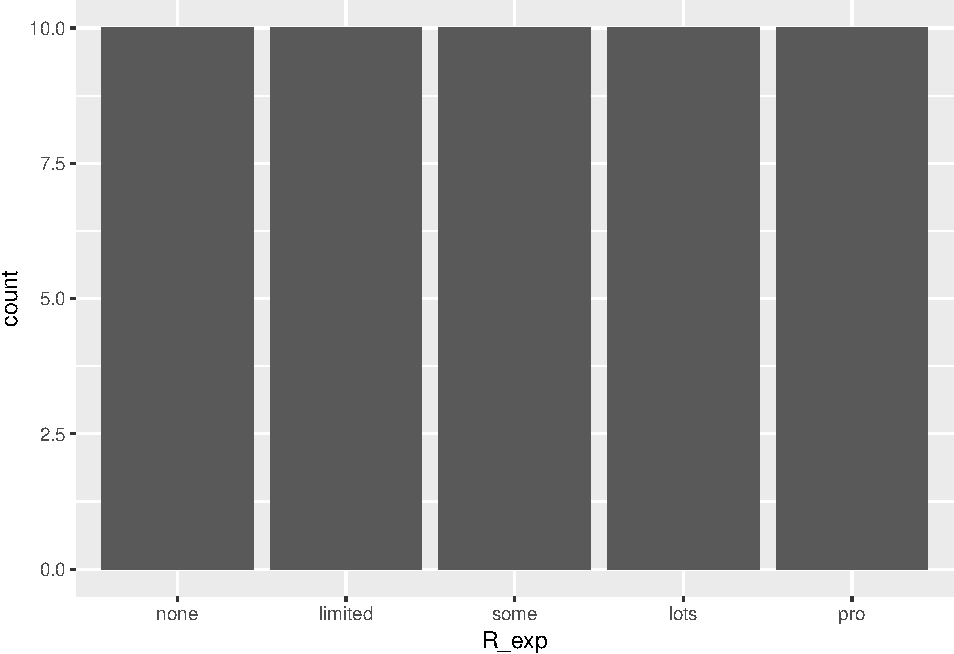
\includegraphics{bootcamp-survey_files/figure-latex/R-exp-hist-1.pdf}
\caption{Distribution of prior R experience}
\end{figure}

\begin{Shaded}
\begin{Highlighting}[]
\NormalTok{Sleep_hrs_hist <-}\StringTok{ }\NormalTok{survey }\OperatorTok
\StringTok{  }\KeywordTok{ggplot}\NormalTok{() }\OperatorTok{+}
\StringTok{  }\KeywordTok{aes}\NormalTok{(}\DataTypeTok{x=}\NormalTok{Sleep_hrs) }\OperatorTok{+}
\StringTok{  }\KeywordTok{geom_histogram}\NormalTok{() }\CommentTok{# Sleep_hrs is continuous}
\NormalTok{Sleep_hrs_hist}
\end{Highlighting}
\end{Shaded}

\begin{verbatim}
## `stat_bin()` using `bins = 30`. Pick better value with `binwidth`.
\end{verbatim}

\begin{figure}
\centering
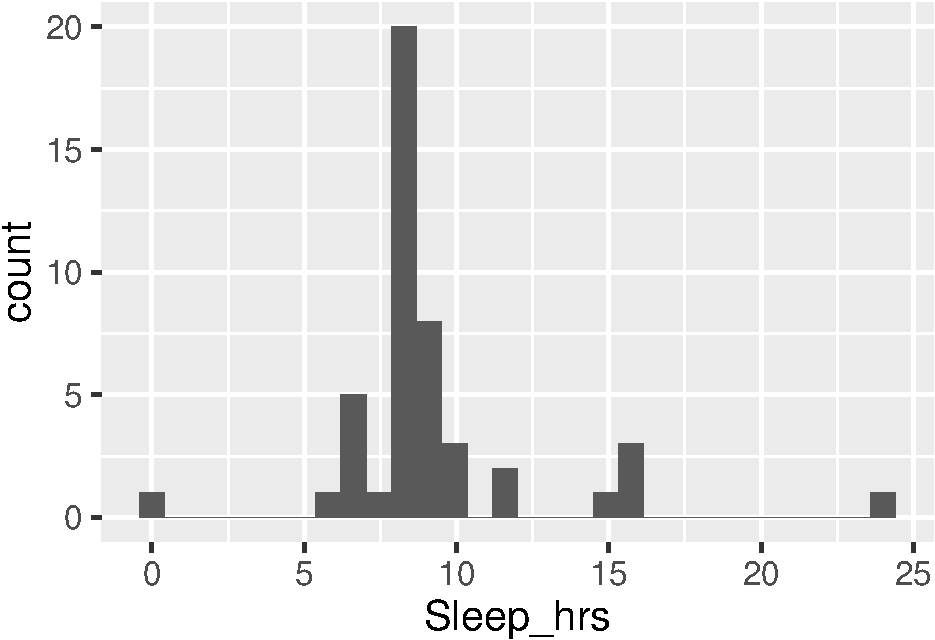
\includegraphics{bootcamp-survey_files/figure-latex/Sleep_hrs_hist-1.pdf}
\caption{Distribution of preferred sleep hrs/day}
\end{figure}

\begin{Shaded}
\begin{Highlighting}[]
\NormalTok{Banjo_hist <-}\StringTok{ }\NormalTok{survey }\OperatorTok
\StringTok{  }\KeywordTok{ggplot}\NormalTok{() }\OperatorTok{+}
\StringTok{  }\KeywordTok{aes}\NormalTok{(}\DataTypeTok{x=}\NormalTok{Banjo) }\OperatorTok{+}
\StringTok{  }\KeywordTok{geom_histogram}\NormalTok{()}
\NormalTok{Banjo_hist}
\end{Highlighting}
\end{Shaded}

\begin{verbatim}
## `stat_bin()` using `bins = 30`. Pick better value with `binwidth`.
\end{verbatim}

\begin{figure}
\centering
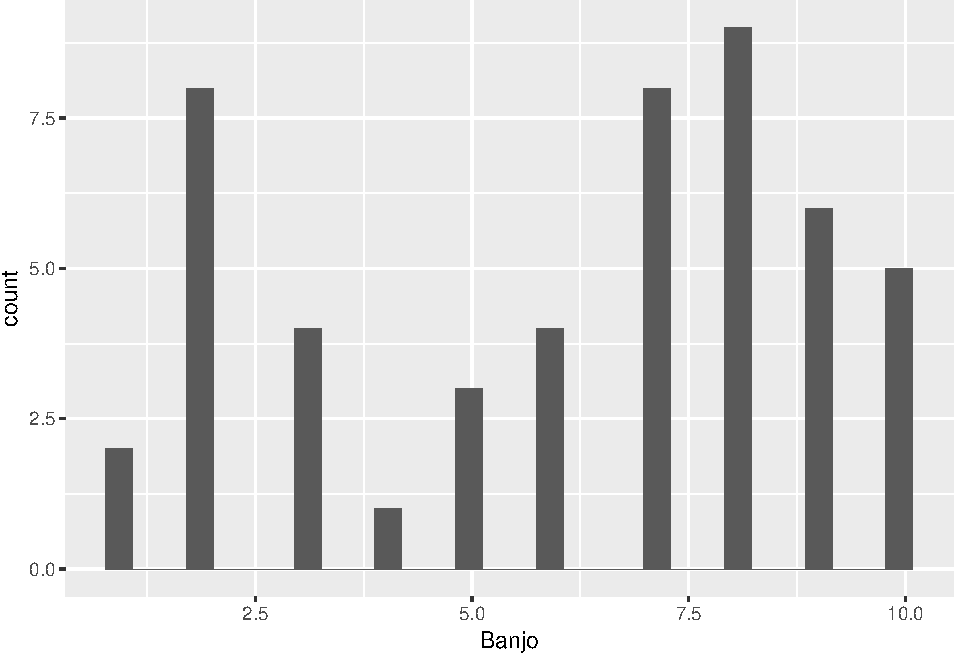
\includegraphics{bootcamp-survey_files/figure-latex/unnamed-chunk-5-1.pdf}
\caption{Distribution of Enthusiasm for Banjo Music}
\end{figure}

\begin{center}\rule{0.5\linewidth}{\linethickness}\end{center}

Does R experience have any relation to banjo music enthusiasm?

\begin{Shaded}
\begin{Highlighting}[]
\NormalTok{Banjo_vs_r_exp <-}\StringTok{ }\NormalTok{survey }\OperatorTok
\StringTok{  }\KeywordTok{ggplot}\NormalTok{() }\OperatorTok{+}
\StringTok{  }\KeywordTok{aes}\NormalTok{(}\DataTypeTok{x=}\NormalTok{Banjo, }\DataTypeTok{y=}\NormalTok{Psych_age_yrs) }\OperatorTok{+}
\StringTok{  }\KeywordTok{facet_grid}\NormalTok{(. }\OperatorTok{~}\StringTok{ }\NormalTok{R_exp) }\OperatorTok{+}
\StringTok{  }\KeywordTok{geom_point}\NormalTok{()}
  \CommentTok{# + stat_smooth()}
\NormalTok{Banjo_vs_r_exp}
\end{Highlighting}
\end{Shaded}

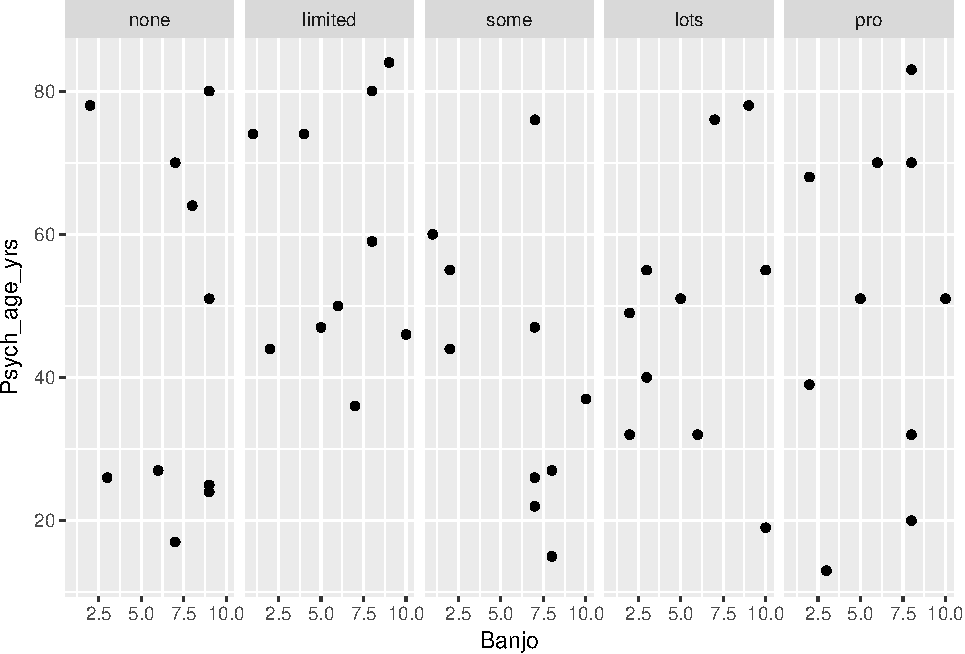
\includegraphics{bootcamp-survey_files/figure-latex/Banjo-vs-r-exp-1.pdf}

\begin{Shaded}
\begin{Highlighting}[]
\NormalTok{crisis_plot <-}\StringTok{ }\NormalTok{survey }\OperatorTok
\StringTok{  }\KeywordTok{ggplot}\NormalTok{() }\OperatorTok{+}
\StringTok{  }\KeywordTok{aes}\NormalTok{(}\DataTypeTok{x=}\NormalTok{Crisis) }\OperatorTok{+}
\StringTok{  }\KeywordTok{geom_bar}\NormalTok{()}
\NormalTok{crisis_plot}
\end{Highlighting}
\end{Shaded}

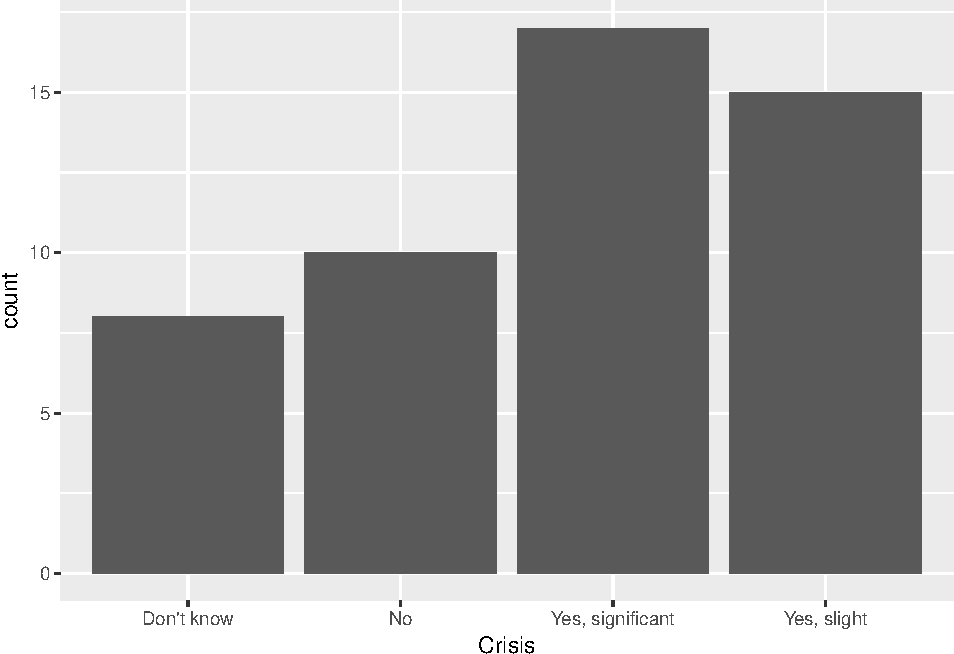
\includegraphics{bootcamp-survey_files/figure-latex/Crisis-1.pdf}

\subsection{Analysis}\label{analysis}

I could use a document like this to plan out my analysis plan
\textbf{before} I conduct it. If I used simulated data, I could make
sure that my workflow will run when I get real (cleaned) data. I could
even preregister my analysis plan before I conduct it. That doesn't
preclude later exploratory analyses, but it does hold me and my
collaborators accountable for what I predicted in advance.

\subsection{Notes}\label{notes}

Notice that I sometimes put a label like \texttt{Banjo-vs-r-exp} in the
brackets \texttt{\{\}}for a given `chunk' of R code. The main reasons to
do this are:

\begin{itemize}
\tightlist
\item
  It sometimes makes it easier to debug your code.
\item
  In some cases, you can have this `chunk' name serve as the file name
  for a figure you generate within a chunk.
\item
  In a bit, we'll see how these chunk names are useful for making
  tables, figures, and equations that generate their own numbers.
\end{itemize}


\end{document}
